\section{Introduction}
Motion Manifold Primitives (MMP) is a generative movement primitive framework based on an autoencoder architecture~\cite{kingma2013auto,hinton2006reducing, bank2023autoencoders}. It encodes a diverse set of trajectories -- collected primarily from human demonstrations -- into a lower-dimensional manifold {\it offline}, thereby enabling {\it online} real-time motion generation and supporting reactive, adaptive behavior in dynamically changing environments~\cite{noseworthy2020task,lee2023equivariant,lee2024mmp++,lee2025motion}.
In this paper, our main objective is to extend this framework to motion generation under stringent kinodynamic constraints, where the generated motions are required to push against the limits of these constraints to successfully accomplish the task (e.g., see Fig.~\ref{fig:intro}).

Throughout, we assume that the objective function and constraints are given -- unlike previous approaches that rely on demonstration data -- so, in principle, a solution could be obtained by solving a trajectory optimization problem.   
However, we focus on problems whose solutions cannot be computed in real time -- specifically, not within sub‑second latency -- due to their complexity and the high dimensionality of the system, despite many advances in sampling, search, and optimization techniques~\cite{chen2020fuzzy,bonalli2019gusto,malyuta2022convex,sakcak2019sampling,yavari2019lazy,atreya2022state,qureshi2021constrained,qureshi2020motion}.


A natural approach is to adapt the MMP framework to our setting by collecting demonstration data through offline trajectory optimization.  
However, existing MMP methods do not explicitly incorporate kinodynamic constraints during training, which often results in trajectories that substantially violate these constraints.



\begin{figure}[!t]
    \centering
    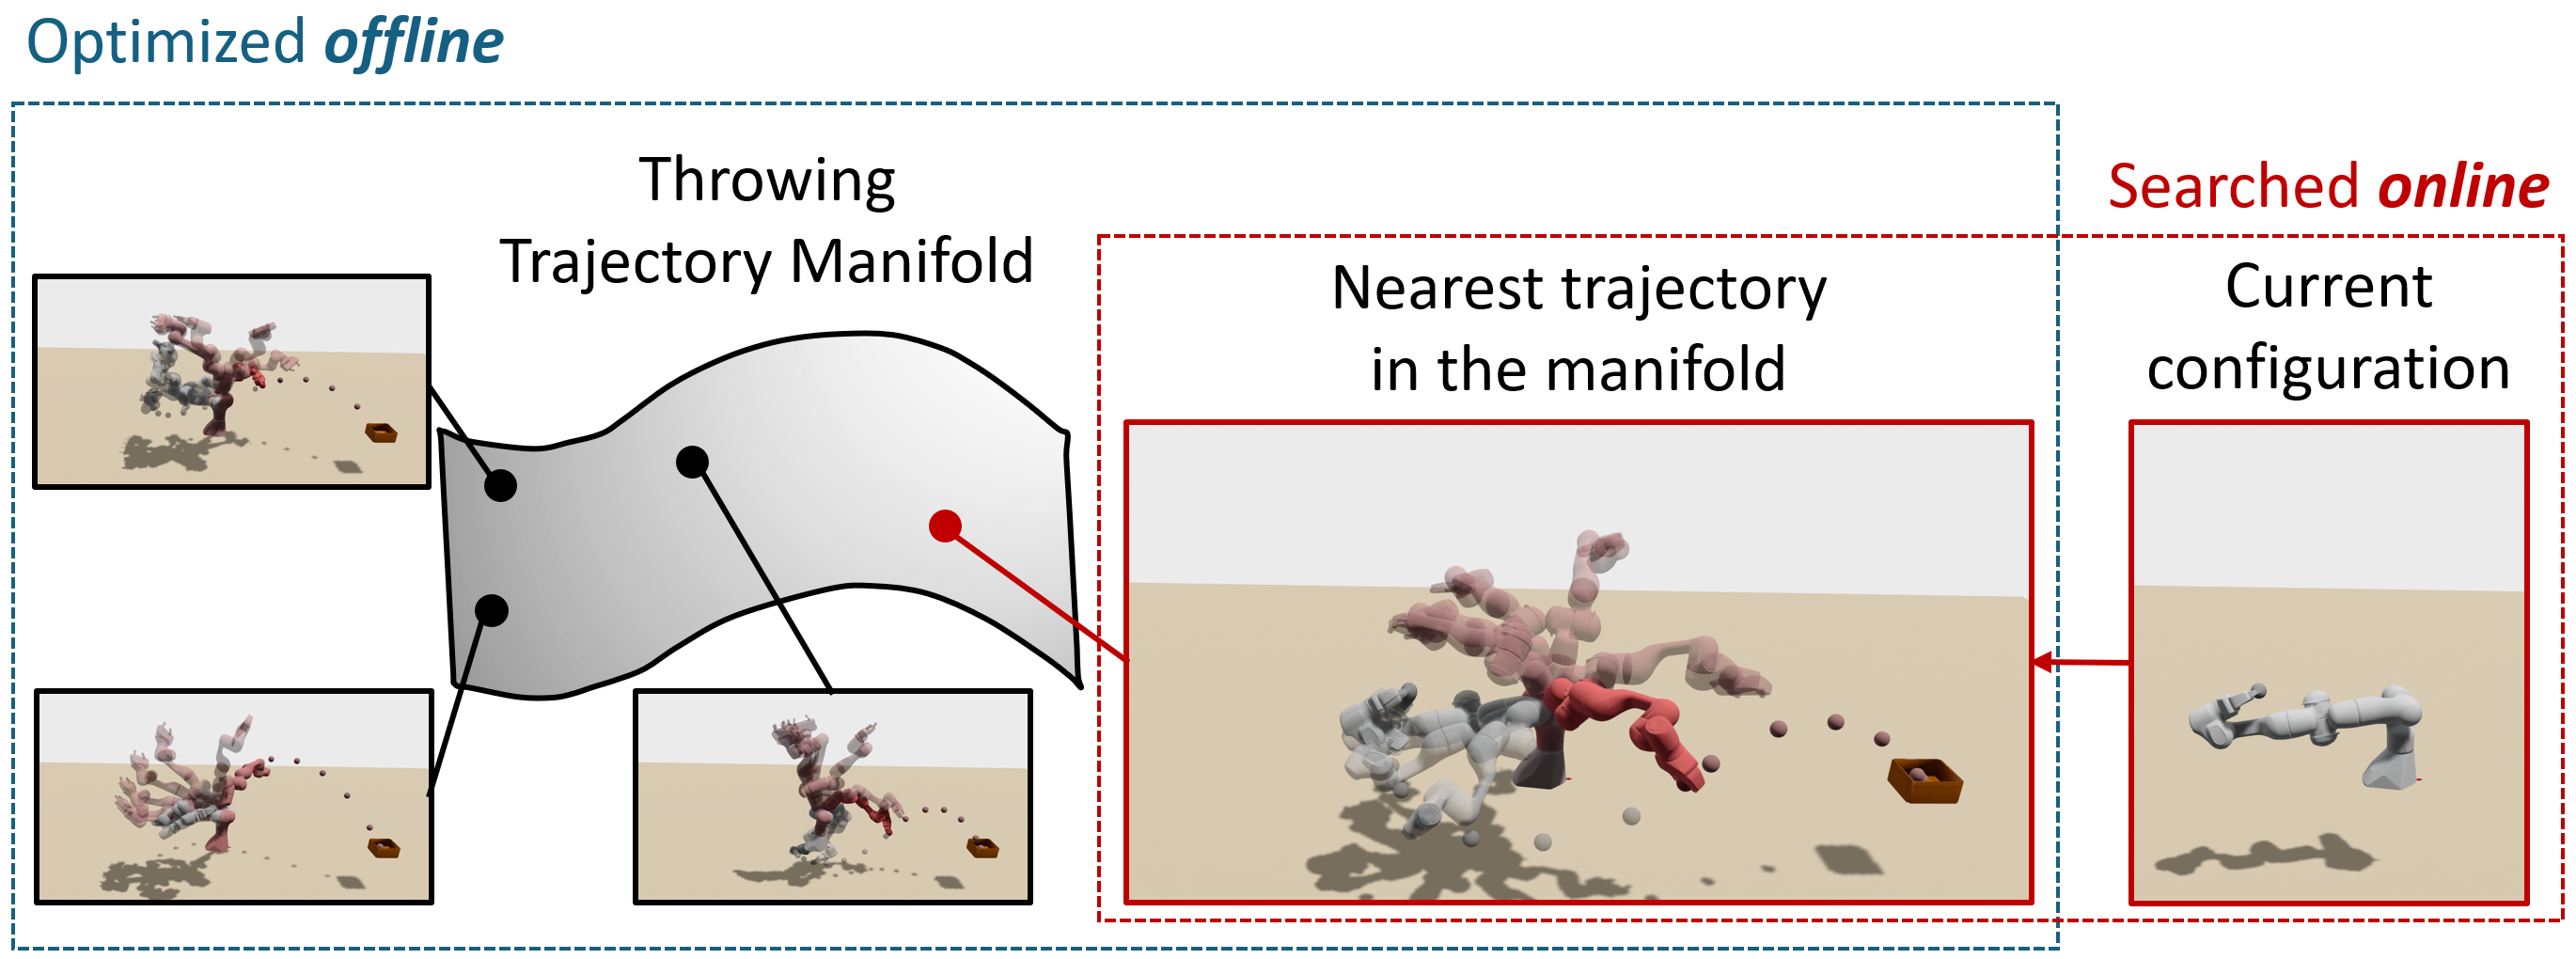
\includegraphics[width=\linewidth]{intro.png}
    \caption{Throwing trajectory manifold -- which consists of task-completing trajectories that satisfy the kinodynamic constraints -- is optimized {\it offline}, and given a current configuration, the nearest throwing trajectory can be quickly searched {\it online} within the manifold. The moment of the throw is depicted in deep red, preceded by gray and followed by transparent red.}
    \label{fig:intro}
    \vspace{-10pt}
\end{figure}

To train an MMP model that satisfies the imposed constraints, we present two key contributions.  
The first is \emph{Differentiable Motion Manifold Primitives (DMMP)}, a novel neural network architecture designed to encode and generate a manifold of continuous‑time trajectories that are differentiable in time.  Unlike prior discrete‑time MMP formulations, this differentiability enables us to naturally enforce constraint satisfaction during training by incorporating the constraints directly into the loss function.
% Generalizing conventional movement primitives~\cite{paraschos2013probabilistic,zhou2019learning}, the DMMP model is formulated as a linear basis‑function model, in which both the basis functions and their coefficients are implemented as neural networks parameterized by latent variables and time, respectively.

The second contribution is a practical four‑step training strategy for DMMP (see Fig.~\ref{fig:summary}; details are provided in Section~\ref{sec:method}).  
First, we collect multiple trajectories for each task parameter by solving trajectory optimization problems with diverse random initializations and seeds.  
Second, we fit these trajectories to a differentiable motion manifold.  
Third, we train a task‑conditioned latent flow model, following~\cite{lee2025motion}.  
Finally, we freeze the latent flow and fine‑tune the manifold to ensure that the generated trajectories both accomplish the tasks and satisfy the kinodynamic constraints.


We present a case study on a dynamic throwing task using a 7‑DoF robot arm, which serves as a representative example of challenging kinodynamic motion‑planning problems.  
To throw beyond the nominal workspace limits, the robot must adopt a preparatory posture -- such as pulling its arm back -- and fully exploit its velocity limits.  
This requires optimizing the entire joint trajectory and the throwing time, rather than only the throwing phase, while simultaneously satisfying kinodynamic constraints, thereby making the problem highly complex.


We compare our DMMP with conventional trajectory optimization methods~\cite{powell1994direct,kraft1988software,kingma2014adam}, as well as existing MMPs~\cite{lee2023equivariant,lee2025motion}, evaluating task success rates, constraint satisfaction rates, and planning times. Our findings demonstrate that our method generates trajectories much more quickly than traditional trajectory optimization, with significantly higher success and constraint satisfaction rates compared to existing MMPs.